\documentclass[tikz]{standalone}
\begin{document}
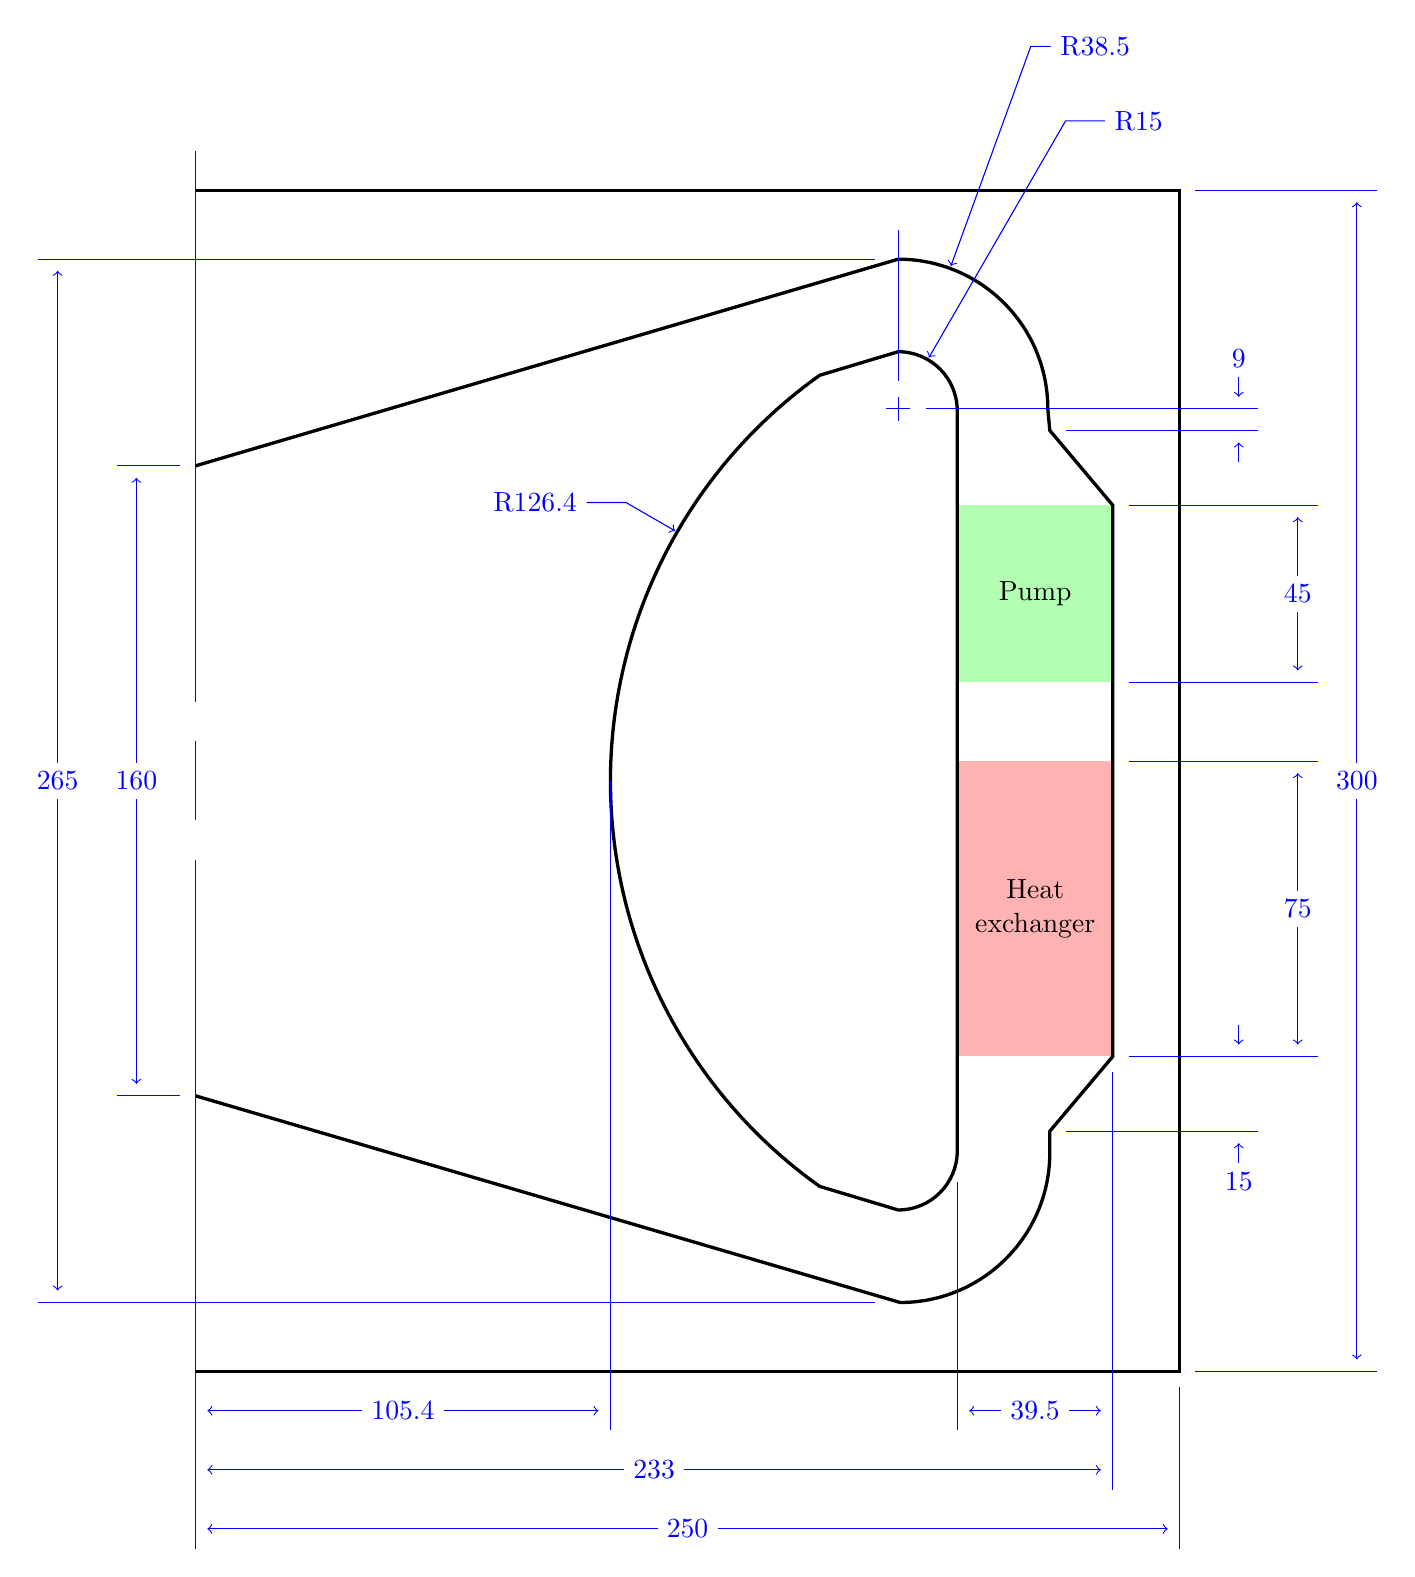
\begin{tikzpicture}
\begin{scope}[scale=5]
  % Shade the pump and heat exchanger regions.
  \fill[green!30!white] (1.935, 0.25) rectangle (2.33, 0.7);
  \fill[red!30!white] (1.935, -0.7) rectangle (2.33, 0.05);
  % Draw the boundaries of the fluid region.
  \draw[very thick] (0, 0.8) -- (1.785, 1.325) arc (90:0:0.38) -- (2.17, 0.89)
    -- (2.33, 0.70) -- (2.33, -0.70) -- (2.17, -0.89) -- (2.17, -0.945)
    arc (0:-90:0.38) -- (0, -0.8);
  \draw[very thick] (1.5857, -1.0302) arc (234.59:125.41:1.264) -- (1.785, 1.09)
    arc (90:0:0.15) -- (1.935, -0.94) arc (0:-90:0.15) -- cycle;
  % Draw the vessel boundaries.
  \draw[very thick] (0, -1.5) -- (2.5, -1.5) -- (2.5, 1.5) -- (0, 1.5);
  % Annotate the pump and heat exchanger.
  \node at (2.133, 0.475) {Pump};
  \node[text width=16mm, align=center] at (2.133, -0.325) {Heat\\exchanger};
  % Draw the reactor centerline.
  \begin{scope}[blue]
    \draw (0, -1.95) -- (0, -0.2) (0, -0.1) -- (0, 0.1) (0, 0.2) -- (0, 1.6);
    % Dimension the minimum core radius.
    \draw (1.054, 0) -- (1.054, -1.65);
    \draw[<->, shorten <=1ex, shorten >=1ex]
      (0, -1.6) -- node[midway, fill=white] {105.4} (1.054, -1.6);
    % Dimension the pump/HX region in the radial direction.
    \draw[shorten <=4mm] (1.935, -0.94) -- (1.935, -1.65);
    \draw[shorten <=2mm] (2.33, -0.7) -- (2.33, -1.8);
    \draw[<->, shorten <=1ex, shorten >=1ex]
      (1.935, -1.6) -- node[midway, fill=white] {39.5} (2.33, -1.6);
    \draw[<->, shorten <=1ex, shorten >=1ex]
      (0, -1.75) -- node[midway, fill=white] {233} (2.33, -1.75);
    % Dimension the vessel in the radial direction.
    \draw[shorten <=2mm] (2.5, -1.5) -- (2.5, -1.95);
    \draw[<->, shorten <=1ex, shorten >=1ex]
      (0, -1.9) -- node[midway, fill=white] {250} (2.5, -1.9);
    % Dimension the core in the axial direction.
    \draw[shorten <=2mm] (0, 0.8) -- (-0.2, 0.8);
    \draw[shorten <=2mm] (0, -0.8) -- (-0.2, -0.8);
    \draw[<->, shorten <=1ex, shorten >=1ex]
      (-0.15, -0.8) -- node[midway, fill=white] {160} (-0.15, 0.8);
    \draw[shorten <=3mm] (1.785, 1.325) -- (-0.4, 1.325);
    \draw[shorten <=3mm] (1.785, -1.325) -- (-0.4, -1.325);
    \draw[<->, shorten <=1ex, shorten >=1ex]
      (-0.35, -1.325) -- node[midway, fill=white] {265} (-0.35, 1.3258);
    % Dimension the core torus minor radius.
    \draw (2.318, 0) ++(150:1.264) -- ++(150:0.15)[<-, shorten <=0.3mm]
      -- ++(-0.1, 0) node[left] {R126.4};
    % Add the centerlines for the hotleg bend.
    \draw (1.785, 0.945) ++(0, -0.03) -- ++(0, 0.06) ++(0, 0.04) -- (1.785, 1.4);
    \draw (1.785, 0.945) ++(-0.03, 0) -- ++(0.06, 0) ++(0.04, 0) -- (2.7, 0.945);
    % Dimension the hotleg bend radii.
    \draw (1.785, 0.94) ++(70:0.385)[<-, shorten <=0.3mm] -- ++(70:0.6)
      -- ++(0.05, 0) node[right] {R38.5};
    \draw (1.785, 0.94) ++(60:0.15)[<-, shorten <=0.3mm] -- ++(60:0.7)
      -- ++(0.1, 0) node[right] {R15};
    % Dimension the straight segment after the hotleg bend.
    \draw[shorten <=2mm] (2.17, 0.89) -- (2.7, 0.89);
    \draw[<-, shorten <=1ex] (2.65, 0.945) -- ++(0, 0.08) node[above] {9};
    \draw[<-, shorten <=1ex] (2.65, 0.89) -- ++(0, -0.08);
    % Dimension the coldleg neck.
    \draw[shorten <=2mm] (2.33, -0.70) -- (2.85, -0.70);
    \draw[shorten <=2mm] (2.17, -0.89) -- (2.7, -0.89);
    \draw[<-, shorten <=1ex] (2.65, -0.7) -- ++(0, 0.08);
    \draw[<-, shorten <=1ex] (2.65, -0.89) -- ++(0, -0.08) node[below] {15};
    % Dimension the gap between the pump and heat exchanger.
    %\draw[shorten <=2mm] (2.33, 0.25) -- (2.7, 0.25);
    %\draw[shorten <=2mm] (2.33, 0.05) -- (2.7, 0.05);
    %\draw[<-, shorten <=1ex] (2.65, 0.25) -- ++(0, 0.08) node[above] {20};
    %\draw[<-, shorten <=1ex] (2.65, 0.05) -- ++(0, -0.08);
    % Dimension the pump and heat exchanger in the axial direction.
    \draw[shorten <=2mm] (2.33, 0.05) -- (2.85, 0.05);
    \draw[<->, shorten <=1ex, shorten >=1ex]
      (2.80, -0.7) -- node[midway, fill=white] {75} (2.80, 0.05);
    \draw[shorten <=2mm] (2.33, 0.25) -- (2.85, 0.25);
    \draw[shorten <=2mm] (2.33, 0.7) -- (2.85, 0.7);
    \draw[<->, shorten <=1ex, shorten >=1ex]
      (2.80, 0.25) -- node[midway, fill=white] {45} (2.80, 0.7);
    %
    \draw[shorten <=2mm] (2.5, 1.5) -- (3.0, 1.5);
    \draw[shorten <=2mm] (2.5, -1.5) -- (3.0, -1.5);
    \draw[<->, shorten <=1ex, shorten >=1ex]
      (2.95, -1.5) -- node[midway, fill=white] {300} (2.95, 1.5);
  \end{scope}
\end{scope}
\end{tikzpicture}
\end{document}
